

\documentclass[10pt,letterpaper]{article}
\usepackage[citations,texMathDollars]{markdown}
\usepackage{cogsci}

\cogscifinalcopy % Uncomment this line for the final submission 


\usepackage{pslatex}
\usepackage{apacite}
\usepackage{float} 
\usepackage{langsci-gb4e}
\usepackage{nnext}
\usepackage{leipzig}
\usepackage{stfloats} 
\usepackage{makecell}

\renewcommand\theadalign{bc}
\renewcommand\theadfont{\bfseries}
\renewcommand\theadgape{\Gape[4pt]}
\renewcommand\cellgape{\Gape[4pt]}


\setlength\titlebox{4.5cm}

\title{Quantifying the cross-linguistics effects of syncretism on agreement attraction}
 
\author{{\large \bf Utku Turk (utkuturk@umd.edu)} \\
  Department of Linguistics, University of Maryland, College Park}


\begin{document}

\maketitle


\begin{abstract}
Speakers' attention to distinctive case markers varies depending on the language they speak. Speakers of languages like German, Russian, or English less often deem ungrammatical sentences grammatical when the case marking is distinctive. However, other languages like Turkish, French, or Armenian do not show this sensitivity, namely additional morphological information provided does not help speakers to create a better representation of the sentence. One explanation for this dichotomy is related to functional utility of morphology in a language. In this study, I first review the psycholinguistic literature on speakers' sensitivity to morphological cues during agreement processing in Turkish, Russian, and English. I then aim to quantify the functional utility of these morphological cues using large language models and their attention patterns. 

\textbf{Keywords:} 
syncretism; agreement attraction; attention; large language models
\end{abstract}

\section{Introduction}


Consider the following sentences in \Next{}.\vspace{-0.5em}

\ea 
    \ea[*]{\label{a}The key to the cabinet are rusty.}\vspace{-0.2em}
    \ex[*]{\label{b}The key to the cabinets are rusty.}\vspace{-0.5em}
    \z
\z

Even though both sentences are ungrammatical due to agreement related reasons, i.e. using `are' instead of `is', psycholinguistic research have shown that speakers are more likely to deem sentences like \xref{b} as grammatical or produce them when the initial preamble includes a plural noun compared to a singular noun \cite{WagersEtAl2009}.

One theory that explains these systematic errors known as agreement attraction is the cue-based retrieval account \cite{WagersEtAl2009}. Following the ACT-R model of sentence processing, this model assumes that words are stored in a content-addressable memory as a chunk that can be later retrieved using specific cues \cite{LewisVasishth2005}. Recall the example in \xref{b}. According to this theory, the noun key would be stored as a following chunk in which the number, the overt case marking, and the dominating syntactic position are encoded: [SG, NOM, TP].\footnote{The selection of which features will be encoded is not exactly clear. The features we present here are not the exclusive list, but rather an exemplary set.} Similarly, the word cabinets would be stored as [PL, NOM, PP].

In the account put forward by \citeA{WagersEtAl2009}, readers would form a prediction based on the chunks they have processed first. In this case, their prediction would be that the agreement carrying element should be singular, given that the noun resides in the syntactic position of an agreement controller [TP] is singular. In cases where participants see `is' or other elements that are singular, no disruption in reading or judgment is seen. On the other hand, if the element they see is `are' or other elements that do not match with the predicted number, a repair process is initiated. In this process, participants would use the relevant cues provided by `are,' such as [PL, NOM, TP], to search for an agreement controller. In \xref{b}, there is no single match, thus most of the time participants do not find these sentences grammatical. However, systematically but occasionally, participants may erroneously retrieve \textit{cabinets} [PL, NOM, PP] as the controller of the agreement due to a partial match between the cues provided by `are.'

On the other hand, this partial match would be a lot less likely to give rise to erroneous retrieval of the word \textit{cabinet} in \xref{a}, since the features shared between the cues of `are' [PL, NOM, TP] and the chunk of `cabinet' [SG, NOM, PP] are even fewer.


\subsection{The role of syncretism}

One crucial assumption shared among the cue-based retrieval models is the role of case marking and morphology \cite{LewisVasishth2005}. In every iteration of the cue-based retrieval theory, the string-based morphological cues are argued to be encoded. For example, in sentences like `I heard you,' even though the syntactic case assigned to `you' is the accusative case, due to the morphological realization the chunk information would include nominative and accusative at the same time. This ambiguity in the morphological output is known to be syncretism. In non-syncretic elements like `he/him,' the case is marked distinctively. Thus, in the sentence `I heard him,' the chunk for the word `him' would contain accusative, but not nominative. 

The role of distinctive case marking is not specific to agreement processes. For example, \citeA{FedorenkoEtAl2004} found that participants were slower to read sentences in sentential embedding configurations like [NP-case NP-case VP VP] when the output of cases are syncretic. The presence of syncretic cases also decreased the overall accuracy of participants in comprehension questions.

\subsection{The effect of syncretism in English Attraction}

Given the role of attractor morphology, one prediction of the cue-based retrieval is that participants should not make similar errors when a possible attractor is marked distinctively. \citeA{NicolEtAl2016} tested this prediction with English possessive marked nouns. Consider the preambles in \Next{}. \vspace{-0.5em}

\ea 
    \ea\label{elfa} The statue in the elf’s garden \ldots{}\vspace{-0.2em}
    \ex\label{elfb} The statue in the elf’s gardens \ldots{}\vspace{-0.2em}
    \ex\label{elfc} The statue in the elves' garden \ldots{}\vspace{-0.2em}
    \ex\label{elfd} The statue in the elves' gardens \ldots{}\vspace{-0.5em}
    \z
\z

They found that participants produced fewer agreement attraction errors with preambles like \xref{elfc} compared to \xref{elfb} or \xref{elfd}. Moreover, there were no significant difference between \xref{elfb} and \xref{elfd}. They took theirs results as an evidence for a confirmation of the use of overt morphological marking in the computation of agreement attraction. 

In another experiment, \citeA{NicolAnton2009} found that using pronouns as attractors as in `\textit{The bill from them} \ldots' diminished the attraction effects compared to sentences with nouns as attractors whose case marking is syncretic between accusative and nominative. Findings of both \citeA{NicolAnton2009} and \cite{NicolEtAl2016} follows from the predictions of the cue based retrieval models.

\subsection{Cross-linguistic picture of syncretism}

However, the effect of syncretism is not clear when one looks at various languages. While certain languages like Turkish or Armenian do not exhibit changes in attraction as a function of case syncretism, other languages like Russian aligns with English and shows increased attraction effects, i.e. more errors in agreement marking, when the forms of the nouns involved in agreement processing is ambiguous. 


% \textbf{German.} \citeA{HartsuikerEtAl2003} provided more direct comparison without use of pronouns or more complex structures. German plural determiners are ambiguous between accusative and nominative `\textit{die}'. However, when dative case is assigned, the determiner surfaces with a distinct form `\textit{den}'. They used the sentence preambles as the ones in \Next{}. Their results showed that participants made more agreement errors while completing sentences with syncretic determiners (\textit{die}), which follows freely from the cue-based retrieval explanation of agreement attraction and retrieval dynamics.

% \ea 
%     \ea\label{ga} Die Stellungnahme zu der Demonstration\\{} 
%     [dative, singular local noun]
%     \ex\label{gb} Die Stellungnahme zu den Demonstrationen\\{} 
%     [dative, plural local noun]
%     \ex\label{gc} Die Stellungnahme gegen die Demonstration\\{} 
%     [accusative, singular local noun]
%     \ex\label{gd} Die Stellungnahme gegen die Demonstrationen\\{} 
%     [accusative, singular local noun]\\
%     The position on (\ref{ga} and \ref{gb}) / against (\ref{gc} and \ref{gd}) the demonstration/s.
%     \z
% \z


\textbf{Russian.} \citeA{Slioussar2018} tested syncretic attractors in Russian, which exhibits an interesting syncretism that is only present in nouns with feminine gender, as in `\textit{statja}' (paper). The singular form of paper when it is marked with a genitive case `\textit{stati}' is syncretic with the plural nominative marked paper `\textit{stati}'. On the other hand, the plural genitive marked paper `\textit{statej}' is distinctively marked and not ambiguous with the nominative plural `\textit{stati}' or singular `\textit{statja}'. She found that when participants were provided with preambles like `\textit{material for paper$_{GEN.SG\ (=NOM.PL)}$}', they made more errors compared to `\textit{material for papers$_{GEN.PL\ (\neq NOM.PL/NOM.SG)}$}'. This effect was robust in both comprehension and production. Her results suggest the string syncretism of case marking can induce the attraction even in cases where the number feature is not plural, which is a stronger version of the tests provided in German and English.


\textbf{Turkish.} Turkish along with Armenian and French differs from previous languages. \citeA{LagoEtAl2019} tested agreement attraction in Turkish by using sentences as in \xref{lago}. However, all the sentences used in their experiment included head nouns `\textit{e\u{g}itmen}' (instructor) that ends with a consonant. The possessive marking in Turkish is syncretic with the accusative case when the noun ends with a consonant. Moreover, the genitive case marked attractor `\textit{teknisyen}' (technician) can be interpreted as a subject of an embedded clause at the time of reading since Turkish embedded subjects are generally marked with a genitive case. \citeA{TurkLogacev2024} tested the role of syncretism in Turkish by minimally changing the the experimental items in \xref{lago}. Instead of using consonant ending head nouns, they used vowel ending head nouns `\textit{hoca}' (teacher) which disambiguated between the accusative case and the possessive marking as in \xref{turk}. They expected that given how syncretism matter in other languages and additionally there is a structural ambiguity in Turkish, using distinctively marked nouns would diminish the attraction effects significantly. However, they found that using distinctive case marking did not affect the magnitude of attraction. Both sentences containing syncretic possessive marking \textit{-i} and distinctive marking \textit{-si} had comparable attraction effects.

\ea \label{lago} 
\gll Teknisyen-(ler)-in e\u{g}itmen-i \ldots{} ko\c{s}tu-(lar).\\
technician-(\Pl{})-\Gen{} instructor-\Poss{} ~ ran-(\Pl{})\\
\glt `The instructor of the technician(s) \ldots{} ran$_{\Sg{}/\Pl{}}$.'
\ex \label{turk} 
\gll Teknisyen-(ler)-in hoca-s{\i} \ldots{} ko\c{s}tu-(lar).\\
technician-(\Pl{})-\Gen{} teacher-\Poss{} ~ ran-(\Pl{})\\
\glt `The teacher of the technician(s) \ldots{} ran$_{\Sg{}/\Pl{}}$.'
\z

\subsection{Quantifying Retrieval}

Is there a way to quantify this retrieval processes and check what happens at each language? The ACT-R model provided by \citeA{LewisVasishth2005} gives the mathematical formulation of such quantification, called \textit{fan} effect. The fan effect is dependent on how many chunks are there and the number of shared features. As the features shared between the chunks increase, the fan effect also increases, and the activation of a chunk decreases. However, for this calculation to go through, one needs to know the which features are tracked. This creates the paradoxical situation, since our main question in this paper is to understand what is different in these languages. One can create a plethora of feature sets and try to explain differences via specific feature engineering. 

Another possible way is to use an approximation. One symptom of the fan effect is the reading times. As the fan effect is increased, it is expected that participants should spend more time to resolve a cue-feature dependency. Recent findings in Deep Neural Network (DNN) suggest that these DNN models can provide quantified numbers, called surprisal values, that can predict humans' reading times in linguistic contexts from 11 different languages \cite{WilcoxEtAl2023}. These 11 languages include English, Russian, and Turkish, which are the languages we test in this paper. If one assumes that the underlying model of human sentence comprehension includes a fan-effect-like mechanism as in cue-based retrieval, it is possible that we can use this approximate number from language models. 


\citeA{RyuLewis2021} recently tested this approximation in English agreement attraction scenarios. They showed that both surprisal values, i.e. how likely a word to appear in a context \cite{Levy2008}, and attention values, i.e. how much importance a specific word in the context carries \cite{ClarkEtAl2019}, predicted the attraction effects in English. In this paper, we are hoping that these values will pattern with presence of absence of attraction effects as a function of case syncretism.



\subsection{Reconciling cross-linguistic facts}

To the best of our knowledge, there is no principled way to explain cross-linguistic facts. One language-specific explanation provided by \citeA{AvetisyanEtAl2020} is that speakers only use case related features for thematic assignment, and they are not used to decide number marking. However, this explanation would fail to explain languages like English, German, or Russian. Another explanation is provided by \citeA{DillonKeshev2024}. They propose that one way to reconcile these opposite cross-linguistic facts is to attribute these differences to language-specific cue dynamics. They raise the possibility that the language-specific utility of morphological cues may underlie the observed effects of syncretism. However, this remains a theoretical proposal, as there is currently no empirical evidence supporting this view. In this work, I am aiming to find evidence for this proposal. If the reason for cross-linguistic differences are due to encoding utility differences, these encoding utility differences might also reveal themselves in suprisal and attention values in LLMs. One would hope that with the amount of data these models are fed, they would be able to pick up distributional facts with respect to case, case syncretism, and the probability of how important morphological information is in controlling dependencies. 

\section{Experimental Setup}

We used the following pretrained models: pre-trained GPT2-small \cite{gpt2} and BERT  \cite{Devlin2018} for English, Turkish-GPT2-small \cite{gptTR} and BERT (\url{https://huggingface.co/dbmdz/bert-base-turkish-cased}) for Turkish, and BERT for Russian (\url{https://huggingface.co/deepvk/bert-base-uncased}). All models were accessed through the \texttt{transformers} or \texttt{minicons} library, and used with the Huggingface API. 

\subsection{Materials}

\begin{table*}[t]
\centering
\caption{Materials used in our simulations. A bold font is used for heads and the attractors are provided underlined.}
\label{tab:materials}
\vspace{0.5em}
\begin{tabular}{llll}
Language & Source & Condition & Sentence \\\hline
English & \citeA{NicolEtAl2016}, Exp3 & Non-Syncretic & The \textbf{statue} in the \underline{elf's/elves'} garden is/*are ...\\
English & \citeA{WagersEtAl2009}, Exp4-7 & Syncretic & The \textbf{key} to the \underline{cabinet/cabinets} is/*are ... \\
Russian & \citeA{Slioussar2018}, Exp3 & Non-Syncretic & \makecell[l]{\textbf{Korobka} dlya \underline{kraski/krasok} byla/*byli ... \\ a box for the paint(s) was/*were ... } \\
Russian & \citeA{Slioussar2018}, Exp3 & Syncretic & \makecell[l]{\textbf{Tropinka} cherez \underline{lug/luga} byla/*byli ... \\ the path through the meadow(s) was/*were ...} \\
Turkish & \citeA{TurkLogacev2024} & Non-Syncretic &  \makecell[l]{\underline{Teknisyennin/Teknisyenlerin} \textbf{hocas{\i}} durmadan ko\c{s}tu/*ko\c{s}tular.\\ The teacher of the technician(s) ran$_{sg}$/*ran$_{pl}$ non-stop.} \\
Turkish & \citeA{LagoEtAl2019} & Syncretic & \makecell[l]{\underline{Teknisyenin/Teknisyenlerin} \textbf{e\u{g}itmeni} durmadan ko\c{s}tu/*ko\c{s}tular.\\ The instructor of the technician(s) ran$_{sg}$/*ran$_{pl}$ non-stop.}\\
\end{tabular}
\end{table*}



We used data from \citeA{TurkLogacev2024} and \citeA{LagoEtAl2019} for Turkish, \citeA{NicolEtAl2016} and \citeA{WagersEtAl2009} for English, and \citeA{Slioussar2018} for Russian. Table \ref{tab:materials} shows the set of experimental sentences as well as their translations. These three sets of sentences have a 2 x 2 x 2 experimental manipulation with the factors grammaticality (grammatical/ungrammatical), number mismatch with the head and the attractor (match/non-match), and case marking (distinctive, non-syncretic/non-distinctive, syncretic) While syncretism (non-distinct case marking) is shown as a different line, other manipulations such as the attractor number and the verb number is shown within the example with slashes. 

\subsection{Metrics}

In this paper, we have used two measures from LLMs: attention to possible agreement controllers and surprisal following \cite{RyuLewis2021}. 

\textbf{Attention.} We extracted the soft attention weights for each relevant noun that could either correctly (grammatical head) or erroneously (attractor) control agreement. We only checked the layer-head combination that has the most likelihood of predicting the subject head. 

\textbf{Surprisal.} We estimated surprisal for the agreement bearing words (auxiliary or main verbs) using two family of models. For GPT-2, we used its left-to-right generation to obtain token-wise surprisal directly. For BERT, which does not predict sequentially, we used masked language modeling: we masked the auxiliary and computed its negative log probability given the surrounding context.


\subsection{Probing heads}

In order to decide which heads to track for agreement related dependencies, we used Universal Dependencies treebanks for English (35,581 total sentences from EWT, GUM, and LinES Treebanks), Turkish (36,760 total sentences from BOUN, Atis, GB, and Kenet Treebanks), and Russian (209,304 total sentences from Taiga and SynTagRus Treebanks). After extracting \texttt{nsubj} dependencies that control dependencies for each sentence, we obtained which attention heads attributed most attention to the element that was tagged with the \texttt{nsubj}. We only used sentences where the subject precedes the verb. Following is the list of layers and attention heads as well as the percentage of these heads paying the highest attention to the subject: English: GPT2: layer4-head11 (36\% accuracy), BERT: layer8-head10 (12\% accuracy), Russian: BERT: layer1-head5 (32\% accuracy), and Turkish: GPT2: layer3-head0 (17\% accuracy), BERT: layer4-head0 (26\% accuracy).


\subsection{Behavioral Results and Predictions}

Our main question is whether an LLM-based approximation for the effects of case-syncretism in agreement attraction is possible. These attraction effects are mainly discussed as differences between plural attractor and singular attractor conditions in ungrammatical sentences (\textit{the key to the cabinets vs. cabinet are}). For this reason, we are going to focus on ungrammatical sentences in our results sections while plots will include values for grammatical sentences too as a control.

Firstly, we should see a difference between the measures as a function of attractor number in Turkish and English only in ungrammatical sentences. In our plots, we will plot the difference ($\Delta$) between Match vs. Mismatch. Since all head nouns are singular, match means a singular attractor, and mismatch means a plural attractor. Assuming that attention to noun phrases in a large language models may reflect the probability of that noun being retrieved as the controller, $\Delta$Head-attention for these languages should be positive and $\Delta$Attractor-attention should be negative, indicating a reduced attention to head but increased attention to attractor in mismatch condition. This differences should get closer to 0 in English, but not change in Turkish as a function of syncretism.

On the other hand, non-syncretic Russian examples should pattern like English, yet, syncretic examples should have a different picture. In syncretic conditions, both match and mismatch condition should have the same sign for the difference: negative for $\Delta$Head and positive for $\Delta$Attractor. These differences should be more amplified for match conditions. 

Secondly, assuming surprisal values reflect reading times as a function of how much features are overlapping between candidates, we expect to see lower surprisal values for mismatch conditions in English and Turkish ungrammatical sentences. This effect should only be visible in non-syretic conditions in Russian. While there is no consistent findings with respect to reading times, the cue-based retrieval account would expect non-syncretic cases to be processed slower, thus increased surprisal values. 

\subsection{Simulation Results}

In the next section, we refer to our plotted descriptive results for each metric and report posteriors' probability of being lower than zero from our maximal Bayesian models fitted to these metrics assuming a lognormal distribution. Our code and data can be found in: \url{https://github.com/utkuturk/syncretism_crossling_llm}.

\paragraph{Attention to head.}

Figure \ref{fig:head-att} shows the attention difference as a function of number mismatch to head metric across 2 models and 3 languages for all 4 conditions: verb number and syncretism. 

In singular verb conditions, the attention to the head does not change as a function of head-attractor number relation ($P(\beta_{Eng} < 0) = 0.53$, $P(\beta_{Ru} < 0) = 0.44$, $P(\beta_{Tr} < 0) = 0.59$), independent of the model type, language, and syncretism. No interactions involving match were significant (all $P(\beta < 0) > 0.11$). This is expected given the general attraction results cross-linguistically. In grammatical sentences (singular verb-singular head), attraction results are rarely observed.  

In plural verb conditions, the picture is slightly different. First of all, our expectation was such that there should be a difference  between the match and mismatch conditions across languages. However, our models revealed a significant main effect of mismatch only in English ($P(\beta < 0) > 0.99$), but not in Russian ($P(\beta < 0) = 0.71$) or Turkish ($P(\beta < 0) = 0.40$). Recall that null main effect is expected in Russian given that both match and mismatch condition induce attraction.

As for our main question, we predicted that mismatch effect should be visible in English syncretic cases. Our model verified this negative interaction: a reliable mismatch effect was found independent of model type ($P(\beta < 0) = 0.09$); however, this interaction was amplified in the BERT model ($P(\beta < 0) = 0.07$). Turkish data showed no evidence for an interaction between match and syncretism ($P(\beta < 0) = 0.44$), which is expected. On the other hand, Russian showed a strong positive evidence for an interaction between match and syncretism ($P(\beta < 0) = 0.98$). This is expected given that syncretic match conditions are found to cause more attraction. 

Overall, we were able to predict English and Russian attraction results and syncretism data. However, we failed to replicate number mismatch difference in Turkish. Even though there were no difference due to syncretism, there were also no baseline attraction-pattern. 

\begin{figure}[htb!]
    \centering
    \vspace*{-1em}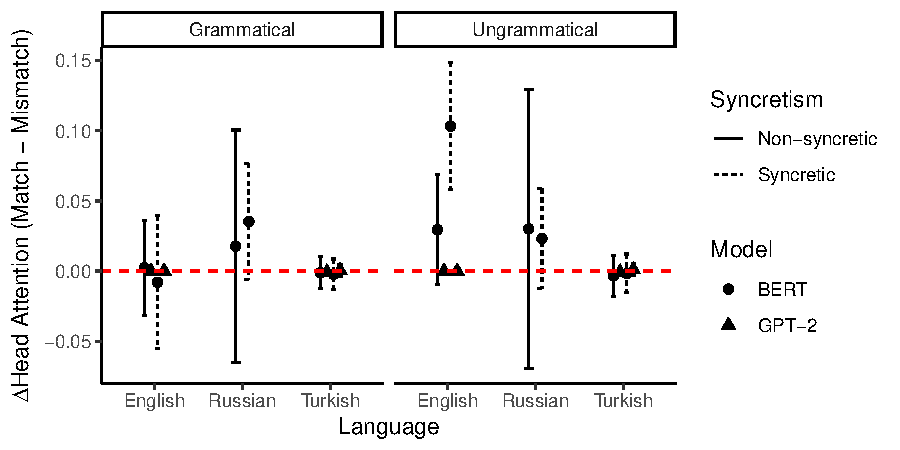
\includegraphics[width=1\linewidth]{p_hatt_diff.pdf}
    \vspace*{-2em}\caption{Head Attention Difference for each language from GPT-2small and BERT models. Error bars signal SE.}
    \label{fig:head-att}
\end{figure}

\vspace*{-2.5em}
\paragraph{Attention to Attractor.}

Figure \ref{fig:att-att} shows the attention difference to attractor metric across the same conditions. One possibility is that even though attention to the head did not change, overall attention to the attractor was funneled from other elements in the sentence and thus was increased. For a cue-based model this would indicate that parser consider non-nominal chunks too. 

As predicted, singular verb (grammatical) conditions do not show any effect as a function of number mismatch ($P(\beta_{Eng} < 0) = 0.54$, $P(\beta_{Ru} < 0) = 0.79$, $P(\beta_{Tr} < 0) = 0.29$). One outlier is Turkish with a BERT language model. There seems to be a more attention allocated to the attractor when both of them are singular ($P(\beta < 0) < 0.001$), as opposed to the mismatch condition where the head is singular and the attractor is plural. 

In the plural verb conditions, BERT models for English and Russian results show a pattern similar to agreement attraction, that is, there is an increased attention to attractors in mismatch conditions (\textit{The key to the cabinets are ...}). Our model verified this effect ($P(\beta_{Eng} < 0) > 0.001$, $P(\beta_{Ru} > 0) = 0.01$). In our plot, this is visible as a negative $\Delta$. Turkish on the other hand showed comparable results to grammatical conditions. 

For our syncretism question, syncretism overall increases the attention to attractor in English ($P(\beta < 0) < 0.99$). More importantly, this attention increase was amplified with number mismatch interaction ($P(\beta < 0) < 0.99$). On the other hand, Russian BERT model did not show such an interaction  ($P(\beta < 0) = 0.34$). This is unexpected mainly because we expected reversed sign for the difference between Match and Mismatch conditions as a function of syncretism. 

Overall, we were able to predict English and Russian attraction data. However, the syncretism related findings were only replicated in English. As for Turkish, even though basic attraction patterns were not found, the insensitivity to morphological form was verified. 

\begin{figure}[htb!]
    \centering
    \vspace*{-1em}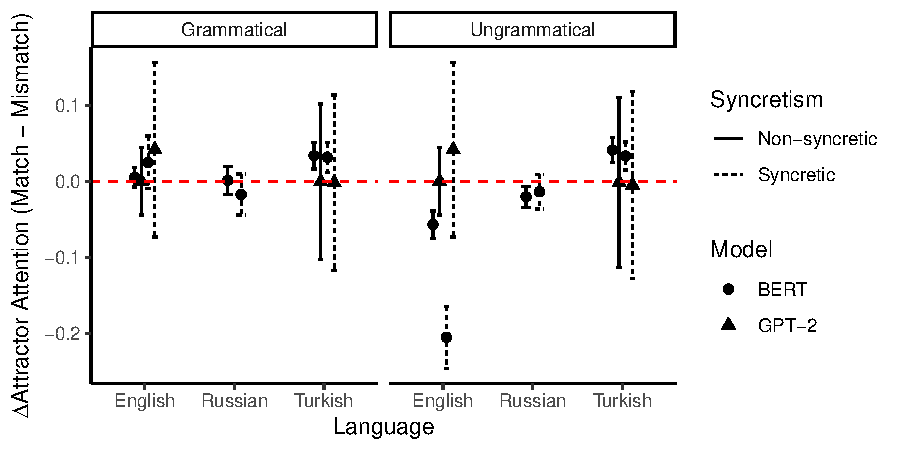
\includegraphics[width=1\linewidth]{p_aatt_diff.pdf}
    \vspace*{-2em}\caption{Attractor attention difference for each language from GPT-2small and BERT models. Error bars signal SE.}
    \label{fig:att-att}
\end{figure}


\vspace{-2em}
\paragraph{Surprisal}

Figure \ref{fig:surp} shows the surprisal difference computed at the auxiliary verbs as a function of number mismatch. It is important to note that even though we have reading data for the Russian data and the syncretic English data, we do not have the reading time data for Turkish or non-syncretic English dataset. However, we will compare our simulation findings to our expectations with minimal additional assumptions. 

Masking-based BERT results shows no effect of number mismatch between the head and the attractor ($P(\beta < 0) = 0.50$) and no interaction with the grammaticality ($P(\beta < 0) = 0.63$), an important pattern observed in  attraction results. Even though there seems to be a difference in surprisal values as a function of syncretism ($P(\beta < 0) < 0.001$), there is also no interaction between the syncretism and the number mismatch ($P(\beta < 0) = 0.48$). 

On the other hand, GPT-2small results reveals an interesting pattern. Firstly, there is no difference as a function of number-mismatch when the verb is singular ($P(\beta < 0) = 0.55$), which is expected given the expectation cue-based model laid on in \citeA{WagersEtAl2009}, meanwhile the vanilla cue-based model would expect increased reading times and thus surprisal with match conditions (singular head-singular attractor-singular verb) due to competition of the cues compared to mismatch conditions.

For the English dataset, we see that surprisal values decreased for the mismatch conditions in non-syncretic nouns when the verb was plural ($P(\beta < 0) > 0.99$  ). For syncretic nouns, surprisal increased slightly in mismatch conditions, signalled with a significant interaction between mismatch and syncretism ($P(\beta < 0) < 0.001$). This aligns with our expectations, since lower surprisal was previously taken to signal decreased reading times. Moreover, previous behavioral results also sugest that reading times decrease in sentences like \textit{the key to the cabinets are ...} compared to \textit{the key to the cabinet are ...}. More importantly, we found that the magnitude of the difference is greater in syncretic conditions  as opposed to non-syncretic conditions. This difference follows from the predictions of cue-based retrieval model. Considering that reading times increase with more features shared between the competitors, it is expected to see lower surprisal in cases with less feature overlap, i.e. no-syncretism cases. Moreover, the fact that there is an interaction between the syncretism and number match is a good sign for the predictability of human behavior with surprisal approximation.

As for Turkish, we again see the effect of number mismatch in the mean surprisal values. As predicted, we see lower surprisal values in mismatch conditions (singular head-plural attractor-plural verb) compared to match conditions (singular head-singular attractor-plural verb) ($P(\beta < 0) < 0.001$). More importantly, the syncretism does not have an effect on the difference between match and mismatch conditions ($P(\beta < 0) = 0.51$). This is in line with the behavioral findings that shows syncretism does not effect the attraction results. However, there is no direct evidence on reading times in Turkish.

\begin{figure}[htb!]
    \centering
    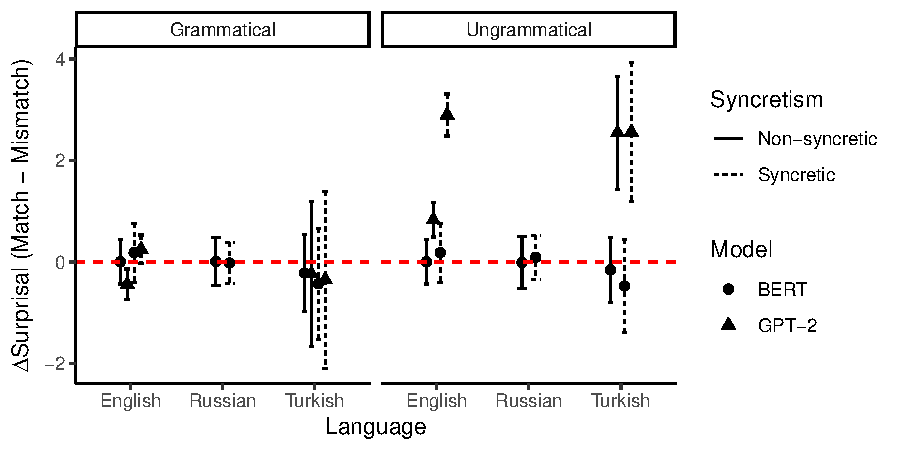
\includegraphics[width=1\linewidth]{p_surp_diff.pdf}
    \vspace*{-2em}\caption{Surprisal values for each model computed at the auxiliary verb. Error bars signal SE.}\vspace*{-2em}
    \label{fig:surp}
\end{figure}




% Check the code 
% Do the stats
% paste them here 
% fix the text
% write up the conclusion


\section{Conclusion}

This paper aimed to quantify, not explain, cross-linguistic facts of morphological form of distinctive case marking using measures from large language models. We specifically tested the agreement attraction sentences. \citeA{DillonKeshev2024} suggest that cross-linguistic differences might be due to the functional informativity of morphological marking in a specific language. Following the link proposed by \citeA{RyuLewis2021}, we argued that attention values are linked to likelihood of memory retrieval which is based on the cues utilized, while surprisal values are related to reading times which again depends on cue dynamics. 

We were able to predict the behavioral findings in English in both surprisal values and attention values. We were also able to predict morphological insensitivity in Turkish, even though the attraction patterns in attention measure were not conclusive. Finally, we were able to predict Russian attraction findings, but not the effect of morphological manipulation with none of the models. 

One of the reasons for this might be due to the very low attention head accuracy. We only used hand-annotated data for head-probing. A larger data set would prove more useful in increasing the accuracy.

Moreover, we assume that there is one head at play. However, many-to-many relation is also possible given that it is unlikely case is related to syntactic position, choice of preposition, and other semantic features. Moreover, case and number representations are also independent.

Lastly, we leave exploration of this many-to-many relation and explanation of why such a cross-linguistic difference exist in the first place to future studies. We believe that a Counterfactual Intervention method proposed by \citeA{HaoLinzen2023} would prove useful.

% \markdownInput{main.md}

% - Notes: russian bert surprisal should be done this : rubert_surprisal_df["surprisal"] / np.log(2)

% english gpt surpisal is also should be divided by np.log(2)

% stuff that should be fixed

% - head percentages are too low, probably one needs to fit a lot more data to find the most predicting heads.

% - number and syncretism interaction, especially the case marking, probably is not limited to a single vector. a better approach should be thinking about what type of information can be encoded with number and case and one should create a complex vector or mapping of vectors. Then, one can use counterfactual thing to modify it.

\bibliographystyle{apacite}

\setlength{\bibleftmargin}{.125in}
\setlength{\bibindent}{-\bibleftmargin}

\bibliography{refs.bib}


\end{document}


% This proposal is also not theoretically explored. I believe that there are two different ways that this language-specific utility can arise. Before discussing these ways, I will point out that correlation attention and surprisal values to attraction to reconcile these facts will not differentiate between these methods, but other methods may be used in the future. 

% \textbf{Decreased morpheme importance.} Agglutinative languages like Turkish and Armenian make excessive use of specialized morphemes, unlike Russian, a fusional language. \citeA{BickelNichols2013} report that a Turkish verb may have up to 9 inflectional morphology, meanwhile this number is up to 4 for Russian, and 1 for English. Therefore, it is possible that one extra morphological cue has less of an effect in agglutinative languages like Turkish compared to languages like English where the number of morphemes is very limited. 
    
% \textbf{Coarseness of features.} In a set of papers, \citeA{BhatiaBrian2022}, as well as \citeA{Bleotu2024}, explored whether the driving force behind the agreement is the subject-likeness. This is a version of our question we asked, however, it addresses the question from a different angle. The main assumption in this line of work, the agreement computation relies on a more general heuristic rather than specific case-marking features. This complex general heuristic can be called subject-likeness. How much a phrase is subject/controller-like will depend on many features as well as the case marking given a language. Even though I am not exploring in this paper, a counterfactual intervention analysis would be more appropriate the explore this question \cite{RavfogelEtAl2021,HaoLinzen2023}. After establishing the necessary vector representations for case, word order, syntactic locations, or other important features for subject-likeness, one would be able to find the symmetric representation of such a vector and test if usage of the new vector or multiple vectors would result in more or less attraction.  

% For both of these analyses, one simple prediction for LLMs 
